\documentclass[a4paper, 11pt]{article}
\usepackage[utf8]{inputenc}
\usepackage[english,russian]{babel}
\usepackage[T1, T2A]{fontenc}
\usepackage{graphicx}
\usepackage{multirow}
\usepackage{pgfplots}
\pgfplotsset{compat=1.9}
\usepackage[left = 2cm, right = 2cm, bottom = 2cm, top = 2cm]{geometry}
\usepackage{listings}             % Include the listings-package
\usepgfplotslibrary{groupplots}
\usepackage[top=2cm, left=2cm, right=2cm, left=2cm]{geometry}
\usepackage{amsmath}
\usepackage{threeparttable}
\usepackage[tableposition=top]{caption}
\usepackage{subcaption}
\DeclareCaptionLabelFormat{gostfigure}{Рисунок #2}
\DeclareCaptionLabelFormat{gosttable}{Таблица #2}
\DeclareCaptionLabelSeparator{gost}{~---~}
\captionsetup{labelsep=gost}
\captionsetup[figure]{labelformat=gostfigure}
\captionsetup[table]{labelformat=gosttable}
\renewcommand{\thesubfigure}{\asbuk{subfigure}}
\captionsetup[table]{labelformat=simple, labelsep = endash, justification = raggedright, singlelinecheck = off}
\usepackage{indentfirst}

\graphicspath{{image/}}

\newcommand\tline[2]{$\underset{\text{#1}}{\text{\underline{\hspace{#2}}}}$}

\begin{document}
	\begin{titlepage}
		\centering
		{\fontsize{12pt}{5cm}\selectfont \bfseries Министерство образования и науки Российской Федерации} \\ \vspace{0.5cm}
		{\fontsize{7pt}{5cm}\selectfont ФЕДЕРАЛЬНОЕ ГОСУДАРСТВЕННОЕ АВТОНОМНОЕ ОБРАЗОВАТЕЛЬНОЕ УЧРЕЖДЕНИЕ ВЫСШЕГО ПРОФЕССИОНАЛЬНОГО ОБРАЗОВАНИЯ} \\ 
		\vspace{1cm}
		{\fontsize{12pt}{5cm}\selectfont \bfseries САНКТ-ПЕТЕРБУРГСКИЙ УНИВЕРСИТЕТ ИНФОРМАЦИОННЫХ ТЕХНОЛОГИЙ, МЕХАНИКИ И ОПТИКИ} \\ \vspace{1.5cm}

		{\fontsize{14pt}{5cm}\selectfont Кафедра \hspace{1cm} \underline{Систем Управления и Информатики}  \hspace{1cm} Группа \underline{Р3340}} \\ 
		\vspace{2cm}

		{\fontsize{20pt}{5cm}\selectfont \bfseries Лабораторная работа №8} \\
		{\fontsize{20pt}{5cm}\selectfont \bfseries “Экспериментальное построение областей устойчивости линейной системы на плоскости двух параметров”} \\
		{\fontsize{14pt}{5cm}\selectfont Вариант - 1} \\
		\vspace{1.5cm}

		\flushleft

		{Выполнил \hspace{2cm} \tline{(фамилия, и.о.)}{9cm} (подпись)} \\
		\vspace{2cm}

		{Проверил \hspace{2cm} \tline{(фамилия, и.о.)}{9cm} (подпись)} \\
		\vspace{5cm}

		"\underline{\hspace{0.7cm}}"\hspace{0.2cm}\underline{\hspace{2cm}}\hspace{0.2cm}20\underline{\hspace{0.7cm}}г. \hspace{2cm} Санкт-Петербург, \hspace{2cm} 20\underline{\hspace{0.7cm}}г. \\ \vspace{1cm}

		Работа выполнена с оценкой \hspace{1cm} \underline{\hspace{8cm}} \\ 
		\vspace{1cm}
		Дата защиты "\underline{\hspace{0.7cm}}"\hspace{0.2cm}\underline{\hspace{2cm}}\hspace{0.2cm}20\underline{\hspace{0.7cm}}г.

\end{titlepage}

\begin{center}
\section*{Задание}
\end{center}

\subsection*{Цель работы} 
Ознакомление с экспериментальными методами построения областей устойчивости линейных динамических систем и изучение влияния на устойчивость системы ее параметров.

\subsection*{Исходные данные}
\par
Линейная система третьего порядка, структурная схема которой представлена на рисунке 1:

\begin{figure}[h!]
\center{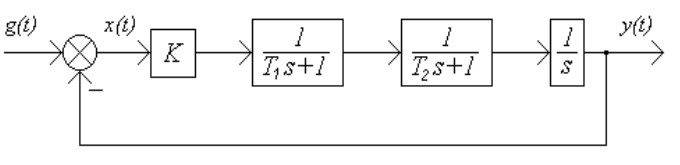
\includegraphics[width=0.75\linewidth]{image/1.png}}
\caption{Структурная схема линейной системы третьего порядка}
\label{ris:image}
\end{figure}

\par 
При этом для варианта определено значение $T_1=0.5c$.

\newpage
\begin{center}
\section{Порядок выполнения лабораторной работы}
\end{center}
\par 
Построим схему моделирования линейной системы третьего порядка в пакете Simulink:

\begin{figure}[h!]
\center{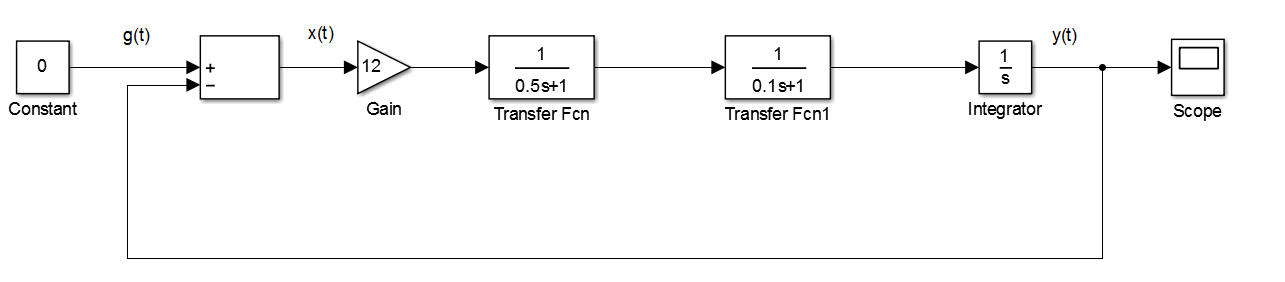
\includegraphics[width=0.75\linewidth]{image/2.png}}
\caption{Схема моделирования линейной системы третьего порядка}
\label{ris:image}
\end{figure}

\par
	Для определения типа устойчивости примем $g(t)=0$ и  $y(0)=1$. Для определения корней характеристического уравнения запишем уравнение связи между входным воздействием и выходной переменной:
\par 
\begin{equation}
\displaystyle (g-y)\frac{K}{s(T_1s+1)(T_2s+1)}=y
\end{equation}

\par 
При условии, что $g(t)=0$ и $T_1=0.5c$, получим:
\par 
\begin{equation}
\displaystyle y\frac{K}{s(0.5s+1)(T_2s+1)}+y=0
\end{equation}

\par 
\begin{equation}
\displaystyle s(0.5s+1)(T_2s+1)y+Ky=0
\end{equation}

\par 
\begin{equation}
\displaystyle 0.5T_2s^3y+(T_2+0.5)s^2y+sy+Ky=0
\end{equation}

\par 
Это эквивалентно следующему дифференциальному уравнению:
\par 
\begin{equation}
\displaystyle 0.5T_2y^{(3)}+(T_2+0.5)y^{(2)}+y^{(1)}+Ky=0
\end{equation}

\par 
Характеристическое уравнение будет иметь следующий вид:
\par 
\begin{equation}
\displaystyle 0.5T_2y^{(3)}+(T_2+0.5)y^{(2)}+y^{(1)}+Ky=0
\end{equation}

\par 
Характеристическое уравнение будет иметь следующий вид:
\par 
\begin{equation}
\displaystyle 0.5T_2s^3+(T_2+0.5)s^2+s+K=0
\end{equation}

\par 
	В схеме моделирования установим  $T_2=0.1 с$ и подберем такое значение $К$, при котором система будет находится на границе устойчивости. Как видно из графика переходного процесса, представленного на рисунке 2, при $K = 12$ система находится на границе устойчивости:

\newpage
\pgfplotsset{
every axis plot post/.append style={
	mark= ,
	every mark/.append style={solid},
	every axis title/.style={at={(0.5,0)},anchor=north,yshift=-0.1}
	}}
На рисунке 3 изображён график выходного сигнала системы, имеющий колебательный характер:
\begin{figure}[h!]
\centering
\begin{tikzpicture}
\begin{axis}[
	xmin = 0,
	xlabel = {\Large{$t,c$}},
	ylabel = {\Large{$y$}},
	width = 250,
	height = 200,
	grid = both,
]

\addplot[line width = 1] table [x=t, y=y] 
              {data/koleb.txt};

\end{axis}
\end{tikzpicture}
\caption{Результаты моделирования при $K=12$, $T_2=0.1$}
\end{figure}

\par 
	В пакете Mathcad найдем корни характеристического уравнения при $T_2=0.1 с$ и $K=12$:

\begin{equation}
v=\left(
\begin{matrix}

K \\
1 \\
T_2+0.5 \\
0.5-T_2 

\end{matrix}
\right)	
\end{equation}

\begin{equation}
polyroots(v)=\left(
\begin{matrix}
-12 \\
-4.472i \\
4.472i
\end{matrix}
\right)
\end{equation}

\par 	
Как видим, присутствуют отрицательные вещественные и чисто мнимые корни, что говорит о том, что система находится на границе устойчивости.
\par 
Теперь подберем такие значения $К$ и $T_2$, при которых система будет неустойчива. Для облегчения оставим прежнее значение $T_2=0.1 с$. Рисунок 4 показывает, что система при $K = 15$ будет неустойчива:

\begin{figure}[h!]
\centering
\begin{tikzpicture}
\begin{axis}[
	xmin = 0,
	xlabel = {\Large{$t,c$}},
	ylabel = {\Large{$y$}},
	width = 250,
	height = 200,
	grid = both,
]

\addplot[line width = 1] table [x=t, y=y] 
              {data/neust.txt};

\end{axis}
\end{tikzpicture}
\caption{Результаты моделирования при $K=15$, $T_2=0.1$}
\end{figure}

\par 
	В пакете Mathcad найдем корни характеристического уравнения при $T_2=0.1 с$ и $K=15$:

\begin{equation}
v=\left(
\begin{matrix}
K \\
1 \\
T_2+0.5 \\
0.5-T_2
\end{matrix}
\right)
\end{equation}

\begin{equation}
polyroots(v)=\left(
\begin{matrix}
-12.348 \\
0.174+4.926i \\
0.174-4.926i 
\end{matrix}
\right)
\end{equation}

\par 
	Как видно, присутствуют отрицательные вещественные комплексно-сопряженные корни с положительной единственной частью, что говорит о наличии в выходной переменной бесконечно возрастающей синусоидальной составляющей.
\par 
	Теперь подберем такие значения $К$ и $T_2$, при которых система будет устойчива. Для облегчения опять оставим прежнее значение $T_2=0.1 с$. Рисунок 5 показывает, что система при $K = 10$ будет устойчива.
\par 
	В пакете Mathcad найдем корни характеристического уравнения при $T_2=0.1 с$ и $K=10$:
\par 
\begin{equation}
v=\left(
\begin{matrix}
K \\
1 \\
T_2+0.5 \\
0.5-T_2
\end{matrix}
\right)
\end{equation}

\begin{equation}
polyroots(v)=\left(
\begin{matrix}
-11.747 \\
-0.127-4.124i \\
-0.127+4.124i 
\end{matrix}
\right)
\end{equation}

\par 
Как видно, вещественные части всех корней отрицательные, что говорит о выполнения условия устойчивости. График устойчивого переходного процесса представлен на рисунке 5. 

\begin{figure}[h!]
\centering
\begin{tikzpicture}
\begin{axis}[
	xlabel = {\Large{$t,c$}},
	ylabel = {\Large{$y$}},
	width = 250,
	height = 200,
	grid = both,
]

\addplot[line width = 1] table [x=t, y=y] 
              {data/ust.txt};

\end{axis}
\end{tikzpicture}
\caption{Результаты моделирования при $K=10$, $T_2=0.1$}
\end{figure}

\par 
Изменяя $T_2$ в диапазоне от $0.1$ с до $5 с$ и подбирая $К$, составим таблицу, необходимую  для построения границы устойчивости. Подобранные с помощью математического моделирования данные приведены в таблице 1.

\newpage
\begin{table}
\centering
\begin{threeparttable}
\caption{Точки построения смоделированной границы устойчивости}\label{tab:perflogcross}
\begin{tabular}{|c|c|c|c|c|c|c|c|c|c|c|c|c|c|}
\hline
$T_2$,c & 0.1 & 0.2 & 0.3 & 0.4 & 0.5 & 1 & 1.5 & 2 & 2.5 & 3 & 3.5 & 4 & 5 \\
\hline
$K$ & 12 & 7 & 5.35 & 4.5 & 4 & 3 & 2.7 & 2.5 & 2.4 & 2.3 & 2.3 & 2.25 & 2.2\\
\hline
\end{tabular}
\end{threeparttable}
\end{table}

\par 
На рисунке 6 представлен график смоделированной границы устойчивости.

\begin{figure}[h!]
\centering
\begin{tikzpicture}
\begin{axis}[
	xlabel = {\Large{$T_2,c$}},
	ylabel = {\Large{$K$}},
	width = 250,
	height = 200,
	grid = both,
]

\addplot[line width = 1] table [x=t, y=y] 
              {data/data.txt};

\end{axis}
\end{tikzpicture}
\caption{График смоделированной границы устойчивости}
\end{figure}

\par 
Матрица Гурвица для системы третьего порядка выглядит следующим образом:
\begin{equation}
M=
\begin{bmatrix}
a_1 & a_3 & 0 \\
a_0 & a_2 & 0 \\
0 & a_1 & a_3 
\end{bmatrix}
\end{equation}

\par 
Подставляя коэффициенты характеристического уравнения, получим:
\begin{equation}
M=
\begin{bmatrix}
T_2+0.5 & K & 0 \\
0.5T_2 & 1 & 0 \\
0 & T_2+0.5 & K
\end{bmatrix}
\end{equation}

\par 
Тогда миноры Гурвица:
\begin{equation}
\Delta_1=T_2+0.5
\end{equation}

\begin{equation}
\Delta_2=
\begin{vmatrix}
T_2+0.5 & K \\
0.5T_2 & 1
\end{vmatrix} 
=T_2+0.5-0.5KT_2
\end{equation}

\begin{equation}
\Delta_3=a_3\Delta_2=K(T_2+0.5-0.5KT_2)
\end{equation}

\par 
По критерию Гурвица запишем условие нейтральной устойчивости системы:

\begin{equation}
\left\{
\begin{matrix}
\Delta_1 & > & 0 \\
\Delta_2 & = & 0 \\
a_3 & > & 0
\end{matrix}
\right. 
\end{equation}
 
\par 
или

\begin{equation}
\left\{
\begin{matrix}
T_2+0.5>0 \\
T_20.5-0.5KT_2=0 \\
K>0
\end{matrix}
\right. 
\end{equation}

\par 
Отсюда:
\begin{equation}
\left\{
\begin{matrix}
T_2>-0.5 \\
\displaystyle K=2+\frac{1}{T_2} \\
K>0
\end{matrix}
\right. 
\end{equation}

\par 
Составим таблицу, необходимую для построения теоретической границы устойчивости. Данные для теоретической границы устойчивости приведены в таблице 2.

\begin{table}
\centering
\begin{threeparttable}
\caption{Точки построения теоретической границы устойчивости}\label{tab:perflogcross}
\begin{tabular}{|c|c|c|c|c|c|c|c|c|c|c|c|c|c|}
\hline
$T_2$,c & 0.1 & 0.2 & 0.3 & 0.4 & 0.5 & 1 & 1.5 & 2 & 2.5 & 3 & 3.5 & 4 & 5 \\
\hline
$K$ & 12 & 7 & 5.33 & 4.5 & 4 & 3 & 2.66 & 2.5 & 2.4 & 2.33 & 2.28 & 2.25 & 2.2\\
\hline
\end{tabular}
\end{threeparttable}
\end{table}

\par 
На рисунке 7 представлена теоретическая граница устойчивости.

\begin{figure}[h!]
\centering
\begin{tikzpicture}
\begin{axis}[
	xlabel = {\Large{$T_2,c$}},
	ylabel = {\Large{$K$}},
	width = 250,
	height = 200,
	grid = both,
]

\addplot[line width = 1] table [x=t, y=y] 
              {data/data_expr.txt};

\end{axis}
\end{tikzpicture}
\caption{График теоретической границы устойчивости}
\end{figure}

\newpage
\begin{center}
\section*{Вывод}
\end{center}
\par 
В ходе лабораторной работы было произведено математическое моделирование границы устойчивости на плоскости двух параметров $(T_2$ и $K$) системы третьего порядка путем анализа переходных процессов системы. Анализ смоделированной  границы устойчивости позволяет сделать вывод о ее гиперболическом характере, т.е. об обратной пропорциональности параметров системы  $T_2$ и $K$. Адекватность смоделированной границы устойчивости проверяется построением теоретической границы через критерий устойчивости Гурвица. Сравнение таблиц построения смоделированной и теоретической границ устойчивости а также анализ их графиков говорит о правильности проведенного в работе моделирования.   
\end{document}
